
 
%%\documentclass[sn-nature]{sn-jnl}% Style for submissions to Nature Portfolio journals
%%\documentclass[sn-basic]{sn-jnl}% Basic Springer Nature Reference Style/Chemistry Reference Style
\documentclass[sn-mathphys,Numbered]{sn-jnl}
\usepackage{graphicx}%
\usepackage{multirow}%
\usepackage{amsmath,amssymb,amsfonts}%
\usepackage{amsthm}%
\usepackage{mathrsfs}%
\usepackage[title]{appendix}%
\usepackage{xcolor}%
\usepackage{textcomp}%
\usepackage{manyfoot}%
\usepackage{booktabs}%
\usepackage{algorithm}%
\usepackage{algorithmicx}%
\usepackage{algpseudocode}%
\usepackage{listings}%
\theoremstyle{thmstyleone}%
\newtheorem{theorem}{Theorem}
\newtheorem{proposition}[theorem]{Proposition}% 

\theoremstyle{thmstyletwo}%
\newtheorem{example}{Example}%
\newtheorem{remark}{Remark}%

\theoremstyle{thmstylethree}%
\newtheorem{definition}{Definition}%

\raggedbottom

\begin{document}

\title[Article Title]{A novel form for Fermi distribution}

%%=============================================================%%
%% Prefix	-> \pfx{Dr}
%% GivenName	-> \fnm{Joergen W.}
%% Particle	-> \spfx{van der} -> surname prefix
%% FamilyName	-> \sur{Ploeg}
%% Suffix	-> \sfx{IV}
%% NatureName	-> \tanm{Poet Laureate} -> Title after name
%% Degrees	-> \dgr{MSc, PhD}
%% \author*[1,2]{\pfx{Dr} \fnm{Joergen W.} \spfx{van der} \sur{Ploeg} \sfx{IV} \tanm{Poet Laureate} 
%%                 \dgr{MSc, PhD}}\email{iauthor@gmail.com}
%%=============================================================%%

\author[1]{\fnm{}\sur{Cheng Tao Yang}}%\email{iauthor@gmail.com}

\author[1,2]{\fnm{} \sur{Martin Formanek}}%\email{iiauthor@gmail.com}
%\equalcont{These authors contributed equally to this work.}

\author[1]{\fnm{} \sur{Johann Rafelski}}%\email{iiiauthor@gmail.com}
%\equalcont{These authors contributed equally to this work.}

\affil[1]{\orgdiv{Department of Physics}, \orgname{The University of Arizona}, \city{Tucson}, \state{Arizona}, \postcode{85721}, \country{USA}}

\affil[2]{\orgdiv{ELI Beamlines Facility}, \orgname{The Extreme Light Infrastructure ERIC}, \orgaddress{ \postcode{252 41}, \city{Dolni Brezany}, \country{Czech Republic}}}

%\affil[3]{\orgdiv{Department}, \orgname{Organization}, \orgaddress{\street{Street}, \city{City}, \postcode{610101}, \state{State}, \country{Country}}}

%%==================================%%
%% sample for unstructured abstract %%
%%==================================%%

\abstract{
We  have identified an innovative approach to express the form of the Fermi distribution, which can be use at low temperatures physics where the Fermi gas remain degenerate and their special feature persist. This novel formulation of Fermi distribution extends the understanding of physics beyond the conventional zero-temperature limit.}


\keywords{Fermi distribution, Low temperature Fermi gas}

%%\pacs[JEL Classification]{D8, H51}

%%\pacs[MSC Classification]{35A01, 65L10, 65L12, 65L20, 65L70}

\maketitle

\section{Introduction}\label{sec1}

In general, the Fermi-Dirac distribution can be written as
\begin{align}
\label{Fermi_exact}
f&=\frac{1}{e^{(E-\tilde{\mu})/T}+1},\qquad\tilde\mu=\pm\mu_e+T\ln\Upsilon
\end{align}
In the extreme limit $T\rightarrow0$, the Fermi-Dirac distribution becomes very simple: a state is either filled or empty. We have
\begin{align}
f&=\frac{1}{e^{(E-\tilde{\mu})/T}+1}=\left\{\begin{array}{c}1,\,\,\,\mathrm{for}\,\,\,{E}<\tilde{\mu} \\0,\,\,\,\mathrm{for}\,\,\, {E}>\tilde{\mu}\end{array}\right.
\end{align}
In general, the energy of the last filled state is called the Fermi energy and is denoted as $E_F$. It is the value of the chemical potential at zero temperature $T=0$, i.e., $E_F=\tilde\mu(T = 0)$. In Fig.~(\ref{Electron_001}) we plot the Fermi-distribution of electron as a function of energy where the parameters are given by $T=0.012\,\mathrm{MeV}$ and chemical potential $\tilde\mu=0.461$ MeV.

%~~~~~~~Figure~~~~~~~~~~~~~~~~~~~~~~~~~~~~~~~~~~~~~
\begin{figure}[h]
\begin{center}
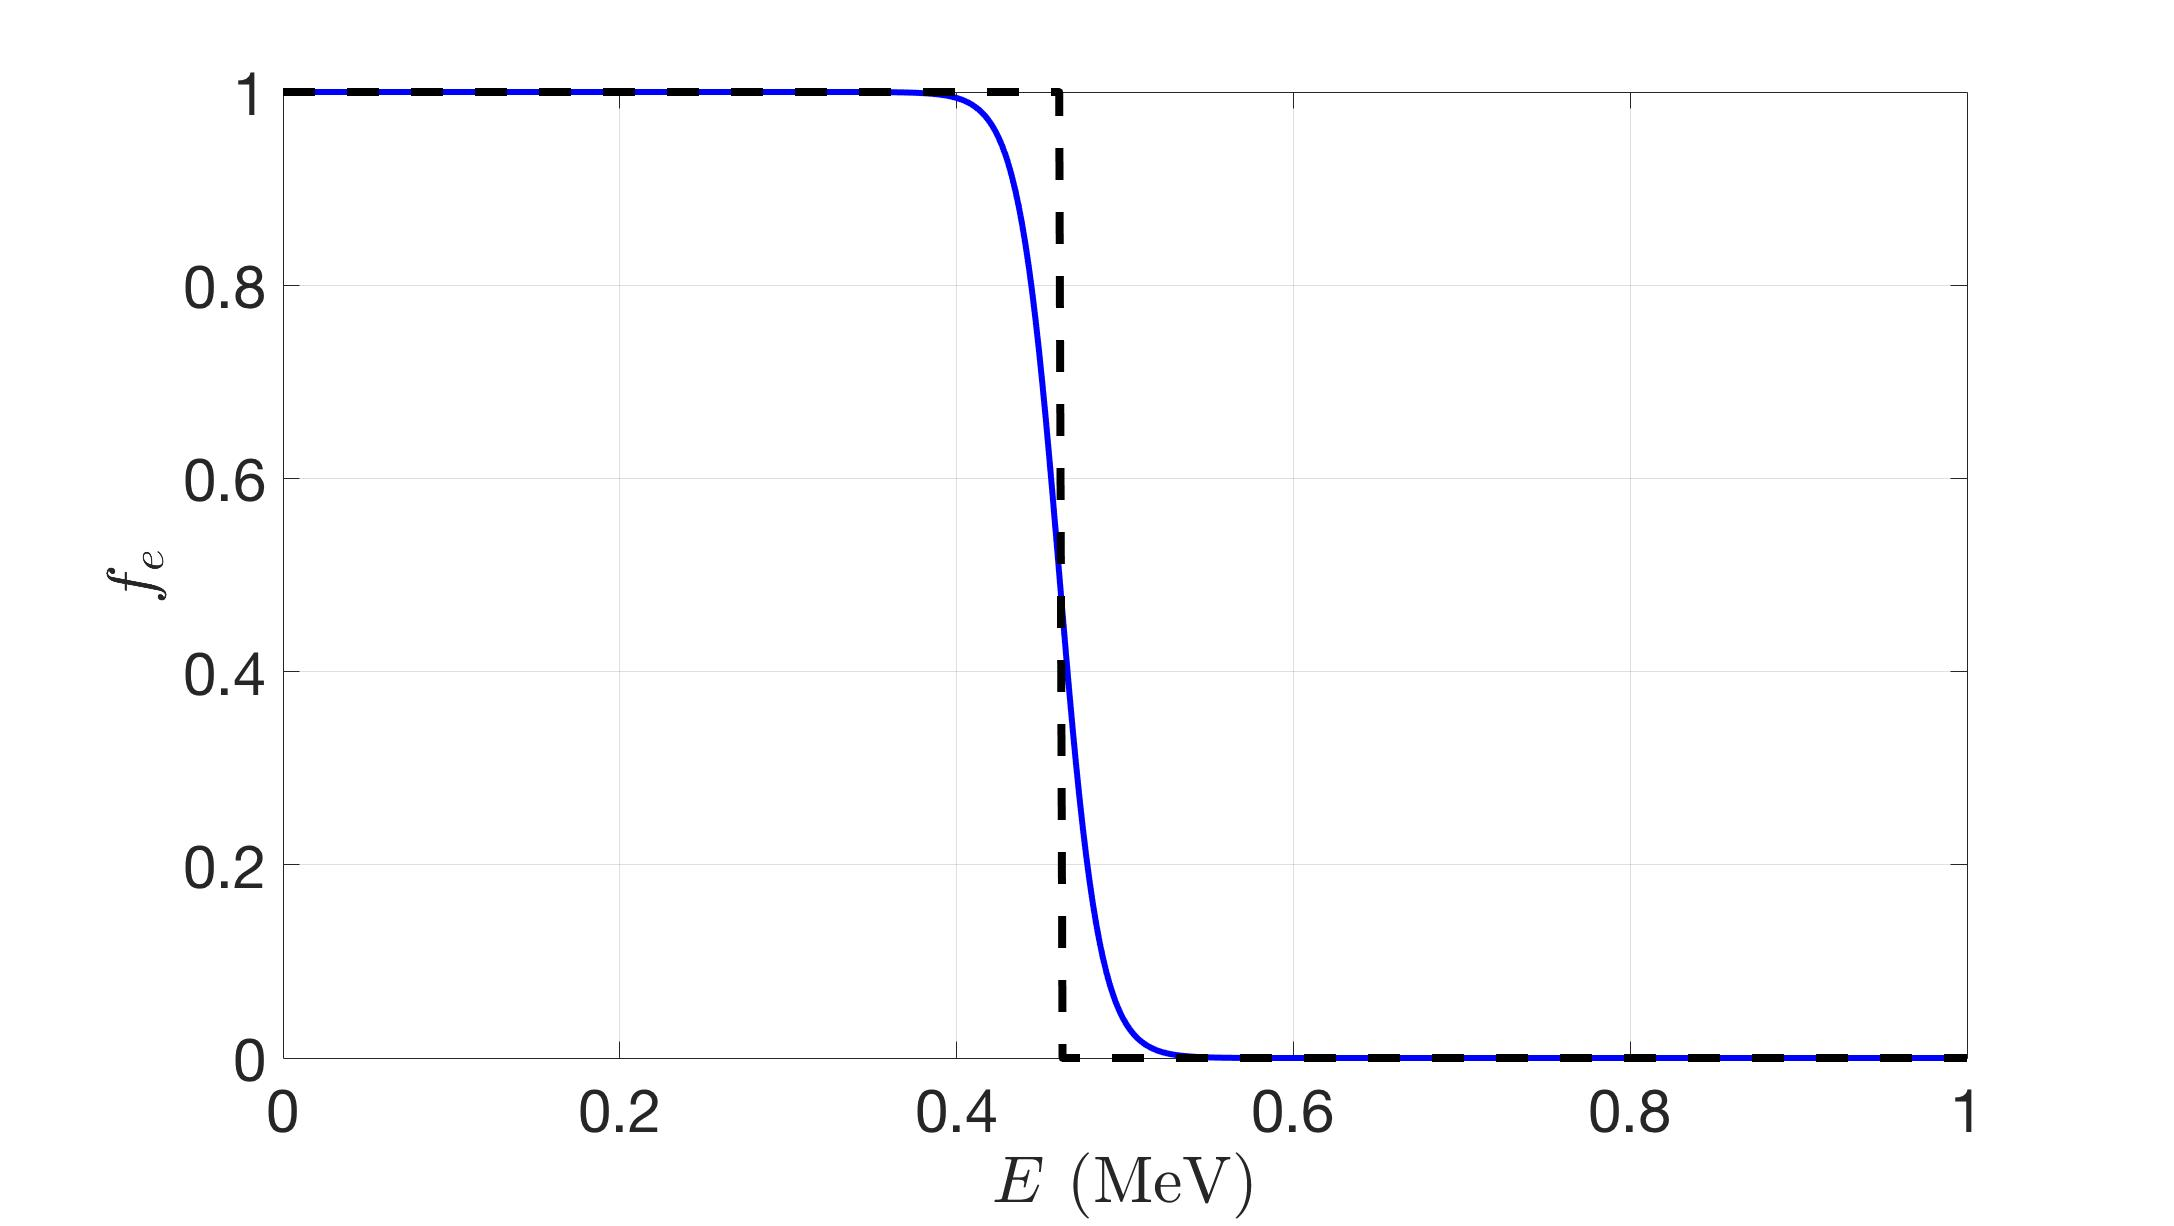
\includegraphics[width=0.9\textwidth]{./plot/Electron_distribution001}
\caption{The Fermi-distribution of electron as a function of energy where the parameters are given by $T=0.012\,\mathrm{MeV}$ and chemical potential $\tilde\mu=0.461$ MeV.}
\label{Electron_001}
\end{center}
\end{figure}
%~~~~~~~~~~~~~~~~~~~~~~~~~~~~~~~~~~~~~~~~~~~~~~~~~~




%%%%%%%%%%%%%%%%%%%%%%%%%%%%%%%%%%%%%%%%%%%%
\section{A new form of Fermi-Distribution}\label{NewFermi}

We have empirically identified the following novel way to state the form of the Fermi distribution. We obtained this form seeking to carry out cosmological computations involving shift in behavior from high to very low-temperature physics. 
\begin{align}\label{NFF1}
f&\equiv \frac{1}{e^{ (E-\tilde\mu)/T} +1}\notag\\
&=\Theta(\tilde\mu - E) +  e^{ - |E-\tilde\mu|/T }
\; \left[\frac{1}{2}\mathrm{sgn}\left({E-\tilde\mu}\right) 
 +\frac{1}{2}\tanh\left(\frac{E-\tilde\mu}{2T}\right)\right]
\end{align}
Note also that the expression in square bracket is a modified form of the sign-function which interpolates between $-1,+1$ for $x\pm \infty$ with a half-unit-sized jump at origin.  We note  that the right hand side (RHS) of Eq.\,(\ref{NFF1}) comprises several non-analytical functions also called distributions. On first sight it is hard to believe that  these   cancel to create the analytical Fermi function format seen on the left hand side (LHS). We will demonstrate that both sides equal to each other.



To demonstrate the novel form of Fermi distribution, we will use the properties of singular functions as follows: 
\begin{align}\label{NFF2a}
\mathrm{sgn}(x)%\equiv \frac{d|x|}{dx}
\equiv  \frac{|x|}{x}\equiv \frac{x}{|x|}\;,
   \quad \mathrm{sgn}(0)=0,\qquad
 \mathrm{sgn}(x)=2\Theta(x)-1\;,
 \end{align}
 and for the step function we use here
 \begin{align}
\label{NFF2c}
 \Theta(x)+\Theta(-x)=1\;,\qquad\label{NFF3}
 \Theta(0)=1/2\;.
 \end{align}
We will need just one complicated expression:
\begin{equation}\label{NFFa1}
\mathrm{sgn}^{2}(x)\sinh(x)=\sinh(x)\;.
 \end{equation}
This is so since $\sinh(x)$  vanishes  at $x=0$ thus we need not worry what value to assign to $\mathrm{sgn}^{2}(x)$ at $x=0$.  

To shorten the notations we define variables as follow
\begin{align}
x^\prime=E-\tilde\mu,\qquad A = \frac{x^\prime}{T}= \frac{E-\tilde\mu}{T}
\end{align}
with these new notations the Fermi function can be written as
\begin{align}
f=\Theta(-x^\prime)+e^{-|A|}\left[\frac{1}{2}\mathrm{sgn}\left(x^\prime\right) 
 +\frac{1}{2}\tanh\left(A\right)\right]
\end{align}
Replacing the step function and exponential function as  follow
 \begin{align}\label{NFF4}
&\Theta(-x^\prime)=\frac 1 2 (1-\mathrm{sgn}(x^\prime))\;,\\ 
&e^{-|A|}=\cosh|A|-\sinh|A|=\cosh A- \mathrm{sgn}(x^\prime)\sinh A\;.
\end{align}
then the Fermi distribution function becomes
\begin{align}
f=\frac{1}{2} &+\left[\cosh {A}- \mathrm{sgn}(x^\prime)\sinh{A} -1\right]\frac{1}{2} \mathrm{sgn}(x^\prime)\notag\\
 &\qquad\qquad\qquad+\left[\cosh{A}- \mathrm{sgn}(x)\sinh{A} \right]\frac{1}{2}\tanh{(A/2)}\;.
\end{align}
Using the properties of singular function  Eq.\,(\ref{NFFa1}), the distribution function can be written as
\begin{align}
f=f_R+f_I
\end{align}
where $f_R$ and $f_I$ represent regular and irregular part of distribution respectively. We have
\begin{align}\label{NFF5a}
 f_R=& \frac{1}{2}\left(1-\sinh A +\cosh A \tanh A/2\right) \\
 f_I=& \mathrm{sgn}(x) \frac{1}{2} \left(\cosh A-1 - \sinh A \tanh A/2\right)
 \label{NFF5b}
\end{align}

For the irregular part $f_I$, we use the properties of hyperbolic functions
\begin{align}
\cosh A-1= 2\sinh^2(A/2), \qquad\sinh A=2 \sinh(A/2) \cosh(A/2)
\end{align}
then it can be written as
\begin{align}
f_I&=\mathrm{sgn}(x) \frac{1}{2} \left[ 2\sinh^2(A/2) - 2 \sinh(A/2) \cosh(A/2) \tanh (A/2)\right]\\
&=\mathrm{sgn}(x) \frac{1}{2}\left[2\sinh^2(A/2)-2\sinh^2(A/2)\right]\\
&=0
\end{align}
we show that the irregular part $f_I$ vanishes as an identity. On the other hand, the regular part $f_R$ can be simplified as below:
\begin{align}
f_R&=\frac{1}{2}\left[1-\frac{1}{2}\left(e^A-e^{-A}\right)+\frac{1}{2}\left(e^A+e^{-A}\right)\frac{e^A-1}{e^A+1}\right]\\
&=\frac{1}{2(e^A+1)}\left[\left(e^A+1\right)-\frac{1}{2}\left[\left(e^A+1\right)\left(e^A-e^{-A}\right)-\left(e^A-1\right)\left(e^A+e^{-A}\right)\right]\right]\\
&=\frac{1}{2(e^A+1)}\left[\left(e^A+1\right)-\left(e^A-1\right)\right]\\
&=f
\end{align}


Finally, we consider the LHS and RHS of Eq.\,(\ref{NFF1}) at $x=0$. With the singular function properties as given we see that at $x=0$ both LHS and RHS of Eq.\,(\ref{NFF1}) are equal to $1/2$ and in the first derivative of the  RHS the two $\delta(x)$-terms 
\begin{align}\label{NFF1b}
\frac{d\Theta(\tilde\mu-E)}{dE}=-\delta(\tilde\mu-E)\;,\qquad 
\frac{d\mathrm{sgn}(E -\tilde\mu)}{dE}=-2\delta(E-\tilde\mu)\;, 
 \end{align}
cancel exactly as required, since there is no $\delta(x)$ on LHS. This encourages us to believe that all of singular expressions cancel. This completes the demonstration of the exact validity of  Eq.\,(\ref{NFF1}). 

In Fig.~(\ref{Fermi_Checking}) we plot the exact Fermi-distribution (LHS of Eq.~(\ref{NFF1}) with solid lines and novel form of Fermi-distribution (RHS of Eq.~(\ref{NFF1})) with dashed lines as a function of energy with different parameters. It demonstrate that 
LHS and RHS of Eq.~(\ref{NFF1}) are equivalent to each other numerically.

%~~~~~~~Figure~~~~~~~~~~~~~~~~~~~~~~~~~~~~~~~~~~~~~~~~~~~~~~~~~~~~~~~~~~~~~~~~~~~~~~~~~~~~~~~~~~~~~
\begin{figure}[h]
\begin{center}
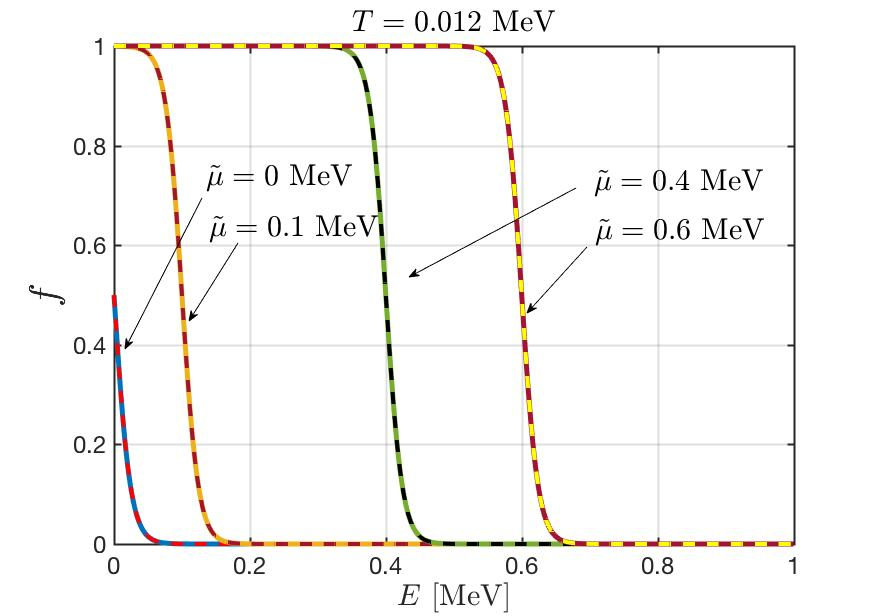
\includegraphics[width=0.5\textwidth]{./plot/Fermi_novel_001}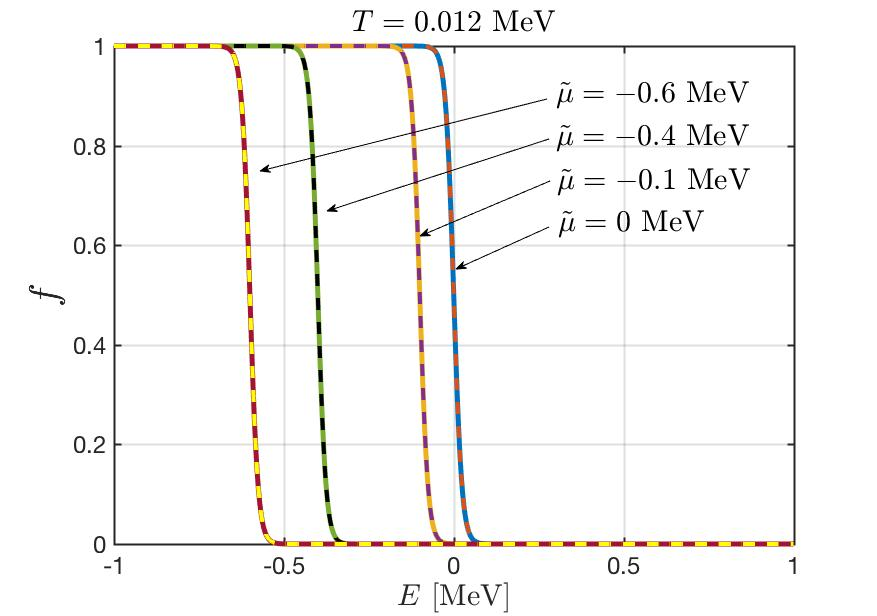
\includegraphics[width=0.5\textwidth]{./plot/Fermi_novel_002}
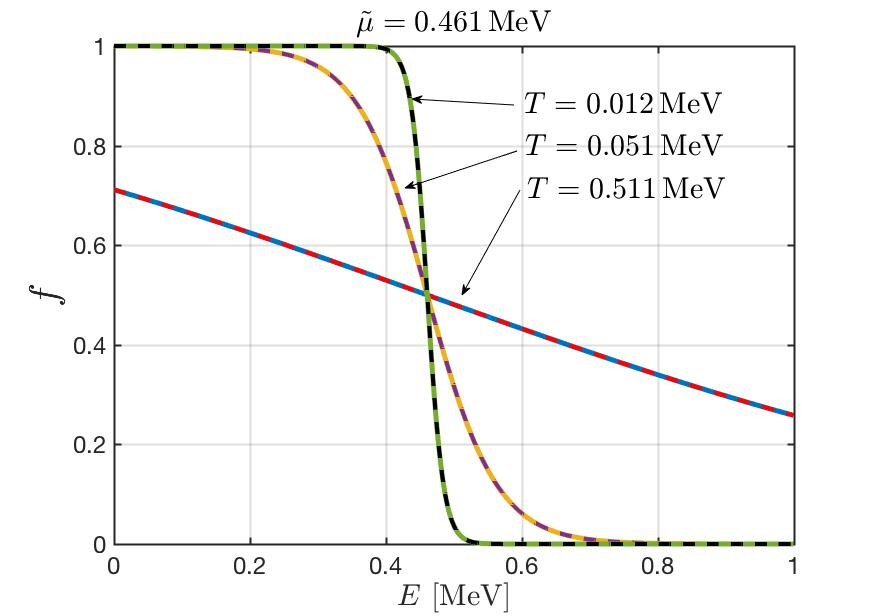
\includegraphics[width=0.5\textwidth]{./plot/Fermi_novel_003}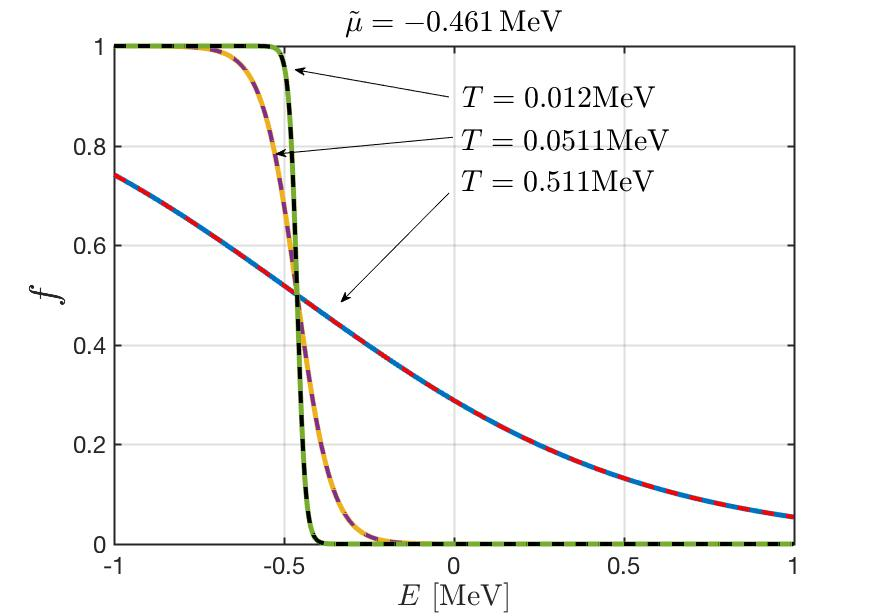
\includegraphics[width=0.5\textwidth]{./plot/Fermi_novel_004}
\caption{The exact Fermi-distribution (LHS of Eq.~(\ref{NFF1}) with solid lines and novel form of Fermi-distribution (RHS of Eq.~(\ref{NFF1})) with dashed lines as a function of energy with different parameters.Top: we compare the RHS and LHS of Eq.~(\ref{NFF1}) with different chemical potential: $\tilde\mu=0, \pm0.1, \pm0.4\,\pm0.6\, \mathrm{MeV}$ at temperature $T=0.012\,\mathrm{MeV}$. Bottom: the Fermi distribution with different temperatures $T=0.511, 0.0511, 0.012\,\mathrm{MeV}$ for chemical potential $\tilde\mu=\pm0.461\,\mathrm{MeV}$.}
\label{Fermi_Checking}
\end{center}
\end{figure}
%~~~~~~~~~~~~~~~~~~~~~~~~~~~~~~~~~~~~~~~~~~~~~~~~~~~~~~~~~~~~~~


%%%%%%%%%%%%%%%%%%%%%%%%%%%%%%%%%%%%%%%%%%%%%%%%%%%%%%%%%%%%%%%%%%%%%%%%%

\section{Partition function and application}\label{NumericalResult}
In previous section we demonstrate that the Fermi-distribution can be written into a novel form Eq.~(\ref{NFF1}). To illustrate the benefits of our innovative Fermi distribution function in practical applications, it is convenient to rewrite the Fermi-function as \cite{Letessier:2002ony}
\begin{align}
\ln{Z}={gV}\int \frac{d^3p}{(2\pi)^3}\ln(1+\gamma\lambda e^{-\beta E})
\end{align}
where $V$ is the volume, $g$ is the degeneracy factor,$\beta=1/T$,  $\gamma$ is the fugacity parameter and $\lambda=e^{\mu/T}$ is related to chemical potential $\mu$. 

We can simplify the partition function via integrating by parts, we obtain
\begin{align}
\ln{Z}&=gV\frac{\beta}{3}\int \frac{d^3p}{(2\pi)^3}p\frac{\partial E}{\partial p}\frac{1}{\gamma^{-1}\lambda^{-1}e^{\beta E}+1}\\
&=\frac{V}{3T}\frac{g}{2\pi^2}\int^\infty_m\,dE\left(E^2-m^2\right)^{3/2}\frac{1}{e^{(E-\tilde\mu)T}+1}
\end{align}
where we introduce the the general chemical potential $\tilde\mu$ as follow
\begin{align}
\tilde\mu=\mu+T\ln\gamma.
\end{align}
To evaluate the partition function, it is convenient to rewrite the Fermi-function as 
\begin{align}
f=f_{\mathrm{cold}} +f_\delta+f_\epsilon.
\end{align}
where the function $f_{\mathrm{cold}}$, $f_{\delta}$, and $f_{\epsilon}$ are defined as
\begin{align}
&f_{cold}=\Theta(\tilde\mu-E),\\
&f_{\delta}=\frac{1}{2}\frac{(E-\tilde\mu)}{|E-\tilde\mu|}\,e^{-|E-\tilde\mu|/T},\qquad f_{\epsilon}=\frac{1}{2}e^{-|E-\tilde\mu|/T}\,\tanh\bigg[\frac{E-\tilde\mu}{2T}\bigg]
\end{align}
In this case, the partition function of Fermi gas can be written as
\begin{align}
\ln{Z}&=\frac{V}{3T}\frac{g}{2\pi^2}\int^\infty_m\,dE\left(E^2-m^2\right)^{3/2}\bigg[f_{cold} +f_\delta+f_\epsilon\bigg]\notag\\
&=\ln{Z}_{\mathrm{cold}}+\ln{Z}_\delta+\ln{Z}_\epsilon
\end{align}
where we define the functions as 
\begin{align}
&\ln{Z}_\mathrm{cold}=\frac{V}{3T}\frac{g}{2\pi^2}\int^\infty_m\,dE\left(E^2-m^2\right)^{{3}/{2}}f_{cold},\\
&\ln{Z}_\delta=\frac{V}{3T}\frac{g}{2\pi^2}\int^\infty_m\,dE\left(E^2-m^2\right)^{3/2} f_\delta,\\
&\ln{Z}_\epsilon=\frac{V}{3T}\frac{g}{2\pi^2}\int^\infty_m\,dE\left(E^2-m^2\right)^{3/2}f_\epsilon
\end{align}
where $\ln Z_{\mathrm{cold}}$ corresponds to the partition function in the limit $T\to 0$, $\ln{Z}_\delta$ and $\ln{Z}_\epsilon$ correspond to terms beyond the conventional
zero-temperature limit. In following we provide the analysis of the integral in detail and show that they can be simplify in the calculation.
%%%%%%%%%%%%%%%%%%%%%%%%%%%%%%%%%%%%%%%%%%%%%%%%%%%%%%%%%%%%%%%%%
%%%%%%%%%%%%%%%%%%%%%%%%%%%%%%%%%%%%%%%%%%%%%%%%%%%%%%%%%%%%%%%%%
\subsection{The partition function of $\ln{Z}_\delta$}
Given the function $f_\delta(E)$ from the Fermi distribution, we have
\begin{align}
f_{\delta}(E)&=\frac{1}{2}\frac{(E-\tilde\mu)}{|E-\tilde\mu|}\,e^{-|E-\tilde\mu|/T},
\end{align}
%~~~~~~~Figure~~~~~~~~~~~~~~~~~~~~~~~~~~~~~~~~~~~~~~~~~~~~~~~~~~~~~~~~~~~~~~~~~~~~~~~~~~~~~~~~~~~~~
\begin{figure}[ht]
\begin{center}
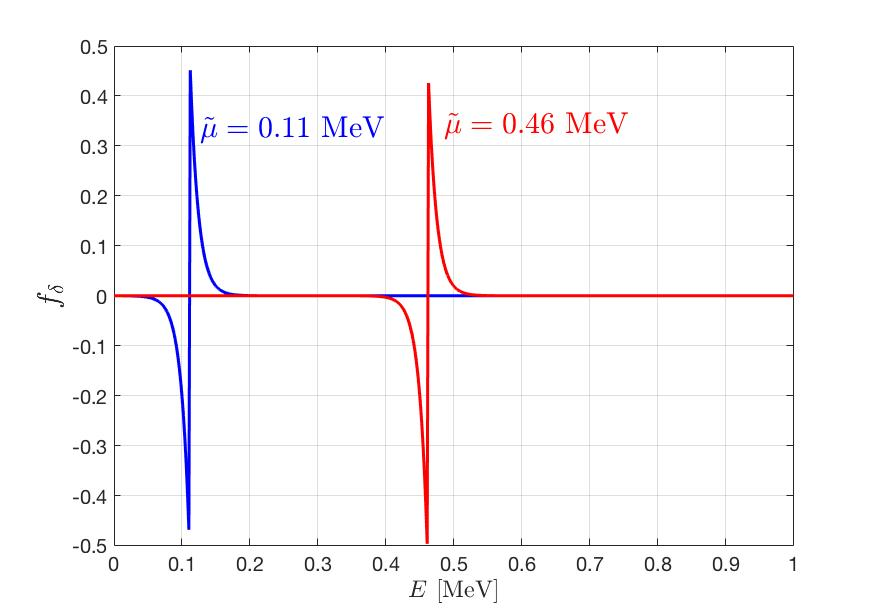
\includegraphics[width=0.9\textwidth]{./plot/f_delta}
\caption{We plot the function $f_\delta$ as a function of energy $E$ at temperature $T=0.012\,\mathrm{MeV}$ with chemical potential $\tilde\mu=0.11\,\mathrm{MeV}$ (blue line), 
 $\tilde\mu=0.46\,\mathrm{MeV}$ (red line). We found that the function has positive and negative peaks at  $E=\tilde\mu$. }
\label{f_delta_graph}
\end{center}
\end{figure}
%~~~~~~~~~~~~~~~~~~~~~~~~~~~~~~~~~~~~~~~~~~~~~
In Fig.(\ref{f_delta_graph}) we plot the function $f_{\delta}(E)$ as a function of energy $E$ at temperature $T=0.012\,\mathrm{MeV}$ with difference chemical potential $\tilde\mu=0.111\,\mathrm{MeV},0.461\,\mathrm{MeV},$. It shows that the function $f_\delta(E)$ has positive and negative peaks at $E=\tilde\mu$.  

Considering the partition function $\ln{Z}_\delta$, it can be written as
\begin{align}
\label{Integral001}
\ln{Z}_\delta&=\frac{V}{3T}\frac{g}{2\pi^2}\int^\infty_m\,dE\left(E^2-m^2\right)^{3/2} \left[\,\frac{1}{2}\frac{(E-\tilde\mu)}{|E-\tilde\mu|}\,e^{-|E-\tilde\mu|/T}\,\right]\notag\\
&=\frac{VT^3}{3}\frac{g}{2\pi^2}\int^\infty_{x_-}\!\!dx\,\left[(x-x_-)(x+x_+)\right]^{3/2}\,\left(\,\frac{1}{2}\frac{x}{|x|}\,e^{-|x|}\,\right),
\end{align}
where in the last step we introduce the dimensionless variable to simplify the integral as below:
\begin{align}\label{Dimensionless}
x\equiv\left({E-\tilde\mu}\right)/T,\qquad x_-=(m-\tilde\mu)/T,\qquad x_+=(m+\tilde\mu)/T.
\end{align}
To evaluate the integral we need to consider the case as follows
\begin{itemize}
  \item Considering $x_->0$, i.e., $m>\tilde\mu$, we have
  \begin{align}
  \ln{Z}_\delta&=\frac{VT^3}{3}\frac{g}{2\pi^2}\int^\infty_{x_-}\!\!dx\,\left[(x-x_-)(x+x_+)\right]^{3/2}\,\left(\,\frac{1}{2}\frac{x}{|x|}\,e^{-|x|}\,\right)\\
  &=\frac{VT^3}{6}\frac{g}{2\pi^2}\int^\infty_{x_-}\!\!dx\,\left[(x-x_-)(x+x_+)\right]^{3/2}\,e^{-x}.
  \end{align}
  In this case, we have the integral with Boltzmann gas distribution and can be evaluated numerically. 
  \item Considering $x_-<0$, i.e., $m<\tilde\mu$, then the partition function can be written as
  \begin{align}
   \ln{Z}_\delta&=\frac{VT^3}{3}\frac{g}{2\pi^2}\int^\infty_{-|x_-|}\!\!dx\,\left[(x+|x_-|)(x+x_+)\right]^{3/2}\,\left(\,\frac{1}{2}\frac{x}{|x|}\,e^{-|x|}\,\right)\\
   &=\frac{VT^3}{6}\frac{g}{2\pi^2}\left[\int^\infty_{|x_-|}\!\!dx\,\left[(x+|x_-|)(x+x_+)\right]^{3/2}\,e^{-x}\right.\notag\\
   &\qquad\qquad\qquad\left.+\int^{|x_-|}_{-|x_-|}\!\!dx\,\left[(x+|x_-|)(x+x_+)\right]^{3/2}\,\frac{x}{|x|}\,e^{-|x|}\right]
  \end{align}
  where the $1$st integral gives us the integral with Boltzmann gas distribution and the $2$md integral provides correction beside the Boltzmann limit.
\end{itemize}
In summary, the partition function $\ln{Z}_\delta$ is given by
\begin{align}
\ln{Z}_\delta&=\frac{VT^3}{6}\frac{g}{2\pi^2}\left[\int^\infty_{|x_-|}\!\!dx\,\left[(x-x_-)(x+x_+)\right]^{3/2}\,e^{-x}\right.\notag\\
   &\qquad\qquad\qquad\left.+\Theta(-x_-)\int^{|x_-|}_{-|x_-|}\!\!dx\,\left[(x+|x_-|)(x+x_+)\right]^{3/2}\,\frac{x}{|x|}\,e^{-|x|}\right],
\end{align}
where we introduce the step function $\Theta(-x_-)$ to include both cases for $x_->0$ and $x_-<0$.
%%%%%%%%%%%%%%%%%%%%%%%%%%%%%%%%%%%%%%%%%%%%%%%%%%%%%%%%%%%%%%%%%

\subsection{The partition function of $\ln{Z}_\epsilon$}
On the other hand, the function $f^{(2)}_\delta(E)$ can be written as (see appendix for detail)
\begin{align}
f^{(2)}_\delta(E)&=\frac{1}{2}\int^{E}_{m}\,dE^\prime\,e^{-|E^\prime-\tilde\mu|/T}\,\tanh\bigg[\frac{E^\prime-\tilde\mu}{2T}\bigg]\notag\\
&=\frac{T}{2}\left[e^{-|\tilde\mu-E|/T}-e^{-|\tilde\mu-m|/T}+2\ln{\left(\frac{1+e^{-|\tilde\mu-m|/T}}{1+e^{-|\tilde\mu-E|/T}}\right)}\right].
\end{align}
In Fig.(\ref{f_delta002_graph}) we plot the function $f_\delta^{(2)}$ as a function of energy $E$ at temperature $T=0.012\,\mathrm{MeV}$ with difference chemical potentials. It shows that the function $f^{(2)}_\delta(E)$ behaves like delta function and has  peaks at $E=\tilde\mu$.
%~~~~~~~Figure~~~~~~~~~~~~~~~~~~~~~~~~~~~~~~~~~~~~~~~~~~~~~~~~~~~~~~~~~~~~~~~~~~~~~~~~~~~~~~~~~~~~~
\begin{figure}[h]
\begin{center}
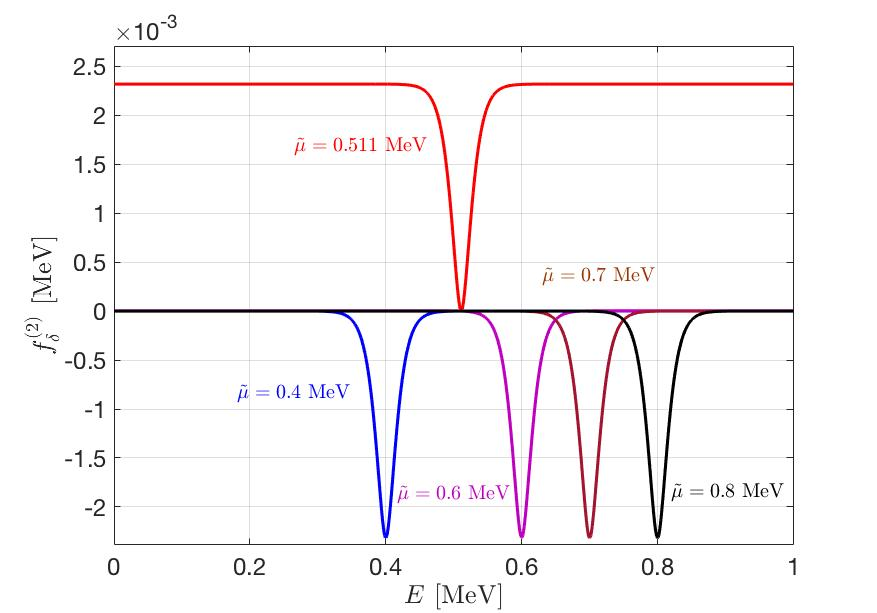
\includegraphics[width=0.9\textwidth]{./plot/f_delta002}
\caption{We plot the function $f^{(2)}_\delta$ as a function of energy $E$ at temperature $T=0.012\,\mathrm{MeV}$ with Fermi-energy around the $m$. We have $\tilde\mu=0.4\,\mathrm{MeV}$ (blue), $\tilde\mu=0.511$ MeV (red), $\tilde\mu=0.6$ MeV (purple), $\tilde\mu=0.7$ MeV (brown),$\tilde\mu=0.8$ MeV (black). We found that the function $f^{(2)}_\delta(E)$ has peaks when the energy  $E=\delta\mu$. }
\label{f_delta002_graph}
\end{center}
\end{figure}
%~~~~~~~~~~~~~~~~~~~~~~~~~~~~~~~~~~~~~~~~~~~~~~~~~~~~~~~~~~~~~~~~~~~~~~~~~~~~~~~~~~~~~~~~~~~~~~~~~

In general, for a given function $g(E)$ the integral for $f_\delta^{(2)}(E)$ is given by
\begin{align}
\label{Integral002}
G_\delta^{(2)}&\equiv\int^\infty_{m}dE\,g^\prime(E)\,f^{(2)}_\delta(E)\notag\\
&=\int^\infty_{m}dE\,g^\prime(E)\frac{T}{2}\bigg[e^{-|\tilde\mu-E|/T}\!-e^{|\tilde\mu-m|/T}\!+2\ln\!\left(\frac{1+e^{-|\tilde\mu-m|/T}}{1+e^{|\tilde\mu-E|/T}}\right)\bigg]\notag\\
&=\frac{1}{2}\int^\infty_{x_0}dx\,g^\prime(x)\bigg[e^{-|x|}-e^{-|x_0|}+2\ln\left(\frac{1+e^{-|x_0|}}{1+e^{-|x|}}\right)\bigg],
\end{align}
where $g^\prime(E)=dg(E)/dE$, and we use the  dimensionless variable Eq. (\ref{Dimensionless}) for the last step. To calculate the integral we need to consider the case as follows
\begin{itemize}
  \item For the case $x_0>0$, i.e., $m>\tilde\mu$, we obtain
  \begin{align}
  G_\delta^{(2)}=&\frac{1}{2}\int^\infty_{x_0}dx\,g^\prime(x)\bigg[e^{-|x|}-e^{-|x_0|}+2\ln\left(\frac{1+e^{-|x_0|}}{1+e^{-|x|}}\right)\bigg]\notag\\
  &=\frac{1}{2}\int^\infty_{x_0}dx\,g^\prime(x)\bigg[e^{-x}-e^{-x_0}+2\ln\left(\frac{1+e^{-x_0}}{1+e^{-x}}\right)\bigg]
  \end{align}
  \item For the case $x_0<0$, i.e., $m<\tilde\mu$, we have
  \begin{align}
   G^{(2)}_\delta&=\frac{1}{2}\int^\infty_{-|x_0|}dx\,g^\prime(x)\bigg[e^{-|x|}-e^{-|x_0|}+2\ln\left(\frac{1+e^{-|x_0|}}{1+e^{-x}}\right)\bigg]\notag\\
   &=\frac{1}{2}\bigg[\left(\int^{|x_0|}_0dx\left(g^\prime(x)+g^\prime(-x)\right)\,e^{-x})+\int^\infty_{|x_0|}dx\,g^\prime(x)\,e^{-|x|}\right)\notag\\
   &+\left(\int^{|x_0|}_0dx\left(g^\prime(x)+g^\prime(-x)\right)\,e^{-|x_0|}+\int^\infty_{|x_0|}dx\,g^\prime(x)\,e^{-|x_0|}\right)\notag\\
&+\left(\int^{|x_0|}_0dx\left(g^\prime(x)+g^\prime(-x)\right)\,2\ln\left(\frac{1+e^{-|x_0|}}{1+e^{-x}}\right)+\int^\infty_{|x_0|}dxg^\prime(x)\,2\ln\left(\frac{1+e^{-|x_0|}}{1+e^{-x}}\right)\right)\bigg]
  \end{align}
\end{itemize}

In both cases, the integral $G^{(2)}_\delta$ can be written as
\begin{align}
G^{(2)}_\delta&=\frac{1}{2}\int^\infty_{x_0}dx\,g^\prime(x)\bigg[e^{-|x|}-e^{-|x_0|}+2\ln\left(\frac{1+e^{-|x_0|}}{1+e^{-|x|}}\right)\bigg]\notag\\
&=\Theta(-x_0)\,\frac{1}{2}\int^{|x_0|}_0dx\,\bigg(g^\prime(x)+g^\prime(-x)\bigg)\bigg[e^{-x}-e^{-|x_0|}+2\ln\left(\frac{1+e^{-|x_0|}}{1+e^{-x}}\right)\bigg]\notag\\
&\qquad+\frac{1}{2}\int^\infty_{|x_0|}dx\,g^\prime(x)\bigg[e^{-x}-e^{-|x_0|}+2\ln\left(\frac{1+e^{-|x_0|}}{1+e^{-x}}\right)\bigg],
\end{align}
where the $1$st integral only exist when the Fermi energy $\tilde\mu>m$ and given function $g^\prime(x)$ is even function. Otherwise we only have the Boltzmann integral.

%%%%%%%%%%%%%%%%%%%%%%%%%%%%%%%%%%%%%%%%%%%%%%%%%%%%%%%%%%%%%%%%%
\subsection{Example: speed of sound}

%%%%%%%%%%%%%%%%%%%%%%%%%%%%%%%%%%%%%%%%%%%%%%%%%%%%%%%%%%%%%%%%%







\section{Results and Discussion}\label{sec12}

 

\backmatter
\section{Appendix: calculation of $f^{(2)}_\delta(E)$ in detail}
The quantity $f^{(2)}_\delta(E)$ can be written as
\begin{align}
\label{f_delta}
f^{(2)}_\delta(E)&=\int^{E}_{m}\,dE^\prime\,\frac{1}{2}\bigg[\Theta(\tilde\mu-E^\prime)\,e^{(E^\prime-\tilde\mu)\beta}+\Theta(E^\prime-\tilde\mu)\,e^{-(E^\prime-\tilde\mu)\beta}\bigg]\,\tanh\bigg[\frac{E^\prime-\tilde\mu}{2T}\bigg]\notag\\
&=\int^{E}_{m}\,dE^\prime\,\frac{1}{2}\bigg[\Theta(\tilde\mu-E^\prime)\,e^{(E^\prime-\tilde\mu)\beta}+\Theta(E^\prime-\tilde\mu)\,e^{-(E^\prime-\tilde\mu)\beta}\bigg]\,\frac{e^{(E^\prime-\tilde\mu)/T}-1}{e^{(E^\prime-\tilde\mu)/T}+1}\notag\\
&=F_1(E)+F_2(E)
\end{align}
where the functions $F_1(E)$ and $F_2(E)$ are defined as
\begin{align}
&F_1(E)=\frac{1}{2}\int^{E}_{m}\,dE^\prime\,\Theta(\tilde\mu-E^\prime)\,e^{(E^\prime-\tilde\mu)\beta}\frac{e^{(E^\prime-\tilde\mu)/T}-1}{e^{(E^\prime-\tilde\mu)/T}+1}\\
&F_2(E)=\frac{1}{2}\int^{E}_{m}\,dE^\prime\,\Theta(E^\prime-\tilde\mu)\,e^{-(E^\prime-\tilde\mu)\beta}\frac{e^{(E^\prime-\tilde\mu)/T}-1}{e^{(E^\prime-\tilde\mu)/T}+1}
\end{align}
To calculate the integrals, it is convenient to compare the $\tilde\mu$ and $m$ first. The function $F_1(E)$ can be written as
\begin{itemize}
\item For $\tilde\mu>E>m$, we have:
\begin{align}
F_1(E)=&\frac{1}{2}\int^{E}_{m}\,dE^\prime\,\Theta(\tilde\mu-E^\prime)\,e^{(E^\prime-\tilde\mu)\beta}\frac{e^{(E^\prime-\tilde\mu)/T}-1}{e^{(E^\prime-\tilde\mu)/T}+1}\\&=\frac{1}{2}\int^{E}_{m}\,dE^\prime\,e^{(E^\prime-\tilde\mu)\beta}\frac{e^{(E^\prime-\tilde\mu)/T}-1}{e^{(E^\prime-\tilde\mu)/T}+1}\notag\\
&=\frac{T}{2}\bigg[e^{-(\tilde\mu-E)/T} -e^{-(\tilde\mu-m)/T} + 2\ln{\left(\frac{1+e^{-(\tilde\mu-m)/T}}{1+e^{-(\tilde\mu-E)/T}}\right)}\bigg]
\end{align}
  \item For $E>\tilde\mu>m$, we have:
\begin{align}
F_1(E)=&\frac{1}{2}\int^{E}_{m}\,dE^\prime\,\Theta(\tilde\mu-E^\prime)\,e^{(E^\prime-\tilde\mu)\beta}\frac{e^{(E^\prime-\tilde\mu)/T}-1}{e^{(E^\prime-\tilde\mu)/T}+1}\\&=\frac{1}{2}\int^{\tilde\mu}_{m}\,dE^\prime\,e^{(E^\prime-\tilde\mu)\beta}\frac{e^{(E^\prime-\tilde\mu)/T}-1}{e^{(E^\prime-\tilde\mu)/T}+1}\notag\\
&=\frac{T}{2}\bigg[(1-\ln4)-e^{-(\tilde\mu-m)/T} + 2\ln{\left(1+e^{-(\tilde\mu-m)/T}\right)}\bigg]
\end{align}
  \item For $E>m>\tilde\mu$, we have:
\begin{align}
F_1(E)=\frac{1}{2}\int^{E}_{m}\,dE^\prime\,\Theta(\tilde\mu-E^\prime)\,e^{(E^\prime-\tilde\mu)\beta}\frac{e^{(E^\prime-\tilde\mu)/T}-1}{e^{(E^\prime-\tilde\mu)/T}+1}=0
\end{align}
\end{itemize}
On the other hand, the second integral in Eq.(\ref{f_delta}) function $F_2(E)$ can be written as
\begin{itemize}
 \item For $\tilde\mu>E>m$, we have:
\begin{align}
F_2(E)=&\frac{1}{2}\int^{E}_{m}\,dE^\prime\,\Theta(E^\prime-\tilde\mu)\,e^{-(E^\prime-\tilde\mu)\beta}\frac{e^{(E^\prime-\tilde\mu)/T}-1}{e^{(E^\prime-\tilde\mu)/T}+1}=0
\end{align}
  \item For $E>\tilde\mu>m$, we have:
\begin{align}
F_2(E)=&\frac{1}{2}\int^{E}_{m}\,dE^\prime\,\Theta(E^\prime-\tilde\mu)\,e^{-(E^\prime-\tilde\mu)\beta}\frac{e^{(E^\prime-\tilde\mu)/T}-1}{e^{(E^\prime-\tilde\mu)/T}+1}\\
&=\frac{1}{2}\int^{E}_{\tilde\mu}\,dE^\prime\,e^{-(E^\prime-\tilde\mu)\beta}\frac{e^{(E^\prime-\tilde\mu)/T}-1}{e^{(E^\prime-\tilde\mu)/T}+1}\notag\\
&=\frac{T}{2}\bigg[(-1+\ln4)+e^{(\tilde\mu-E)/T} -2\ln{\left(1+e^{(\tilde\mu-E)/T}\right)}\bigg]
\end{align}
  \item For $E>m>\tilde\mu$, we have:
\begin{align}
F_2(E)=&\frac{1}{2}\int^{E}_{m}\,dE^\prime\,\Theta(E^\prime-\tilde\mu)\,e^{-(E^\prime-\tilde\mu)\beta}\frac{e^{(E^\prime-\tilde\mu)/T}-1}{e^{(E^\prime-\tilde\mu)/T}+1}\\
&=\frac{1}{2}\int^{E}_{m}\,dE^\prime\,e^{-(E^\prime-\tilde\mu)\beta}\frac{e^{(E^\prime-\tilde\mu)/T}-1}{e^{(E^\prime-\tilde\mu)/T}+1}\notag\\
&=\frac{T}{2}\bigg[e^{(\tilde\mu-E)/T}-e^{(\tilde\mu-m)/T}+2\ln{\left(\frac{1+e^{(\tilde\mu-m)/T}}{1+e^{(\tilde\mu-E)/T}}\right)}\bigg].
\end{align}
\end{itemize}
In this case, the function  $f^{(2)}_\delta$ can be written as
\begin{align}
f^{(2)}_\delta(E)&=F_1(E)+F_2(E)\notag\\
&=\left\{\begin{array}{c}
\frac{T}{2}\left[e^{-(\tilde\mu-E)/T}-e^{-(\tilde\mu-m)/T}+2\ln{\left(\frac{1+e^{-(\tilde\mu-m)/T}}{1+e^{-(\tilde\mu-E)/T}}\right)}\right],\,\,\,\mathrm{for}\,\,\,\,\tilde\mu>E>m \\ 
\frac{T}{2}\left[e^{(\tilde\mu-E)/T}-e^{-(\tilde\mu-m)/T}+2\ln{\left(\frac{1+e^{-(\tilde\mu-m)/T}}{1+e^{(\tilde\mu-E)/T}}\right)}\right],\,\,\,\,\,\,\,\,\mathrm{for}\,\,\,\,E>\tilde\mu>m \\
\frac{T}{2}\left[e^{(\tilde\mu-E)/T}-e^{(\tilde\mu-m)/T}+2\ln{\left(\frac{1+e^{(\tilde\mu-m)/T}}{1+e^{(\tilde\mu-E)/T}}\right)}\right],\,\,\,\,\,\,\,\,\mathrm{for}\,\,\,\,E>m>\tilde\mu
\end{array}\right.
\end{align}
In general, it can be written as
\begin{align}
f^{(2)}_\delta(E)=\frac{T}{2}\left[e^{-|\tilde\mu-E|/T}-e^{-|\tilde\mu-m|/T}+2\ln{\left(\frac{1+e^{-|\tilde\mu-m|/T}}{1+e^{-|\tilde\mu-E|/T}}\right)}\right].
\end{align}
In Fig.(\ref{f_delta_checking}) we plot the function $f^{(2)}_\delta$ as a function of Fermi-energy $E$ for the case $\tilde\mu>m$ . We found that the behavior of $f^{(2)}_\delta$  is like delta function with peak at $E=\tilde\mu$. 
%~~~~~~~Figure~~~~~~~~~~~~~~~~~~~~~~~~~~~~~~~~~~~~~~~~~~~~~~~~~~~~~~~~~~~~~~~~~~~~~~~~~~~~~~~~~~~~~
\begin{figure}[t]
\begin{center}
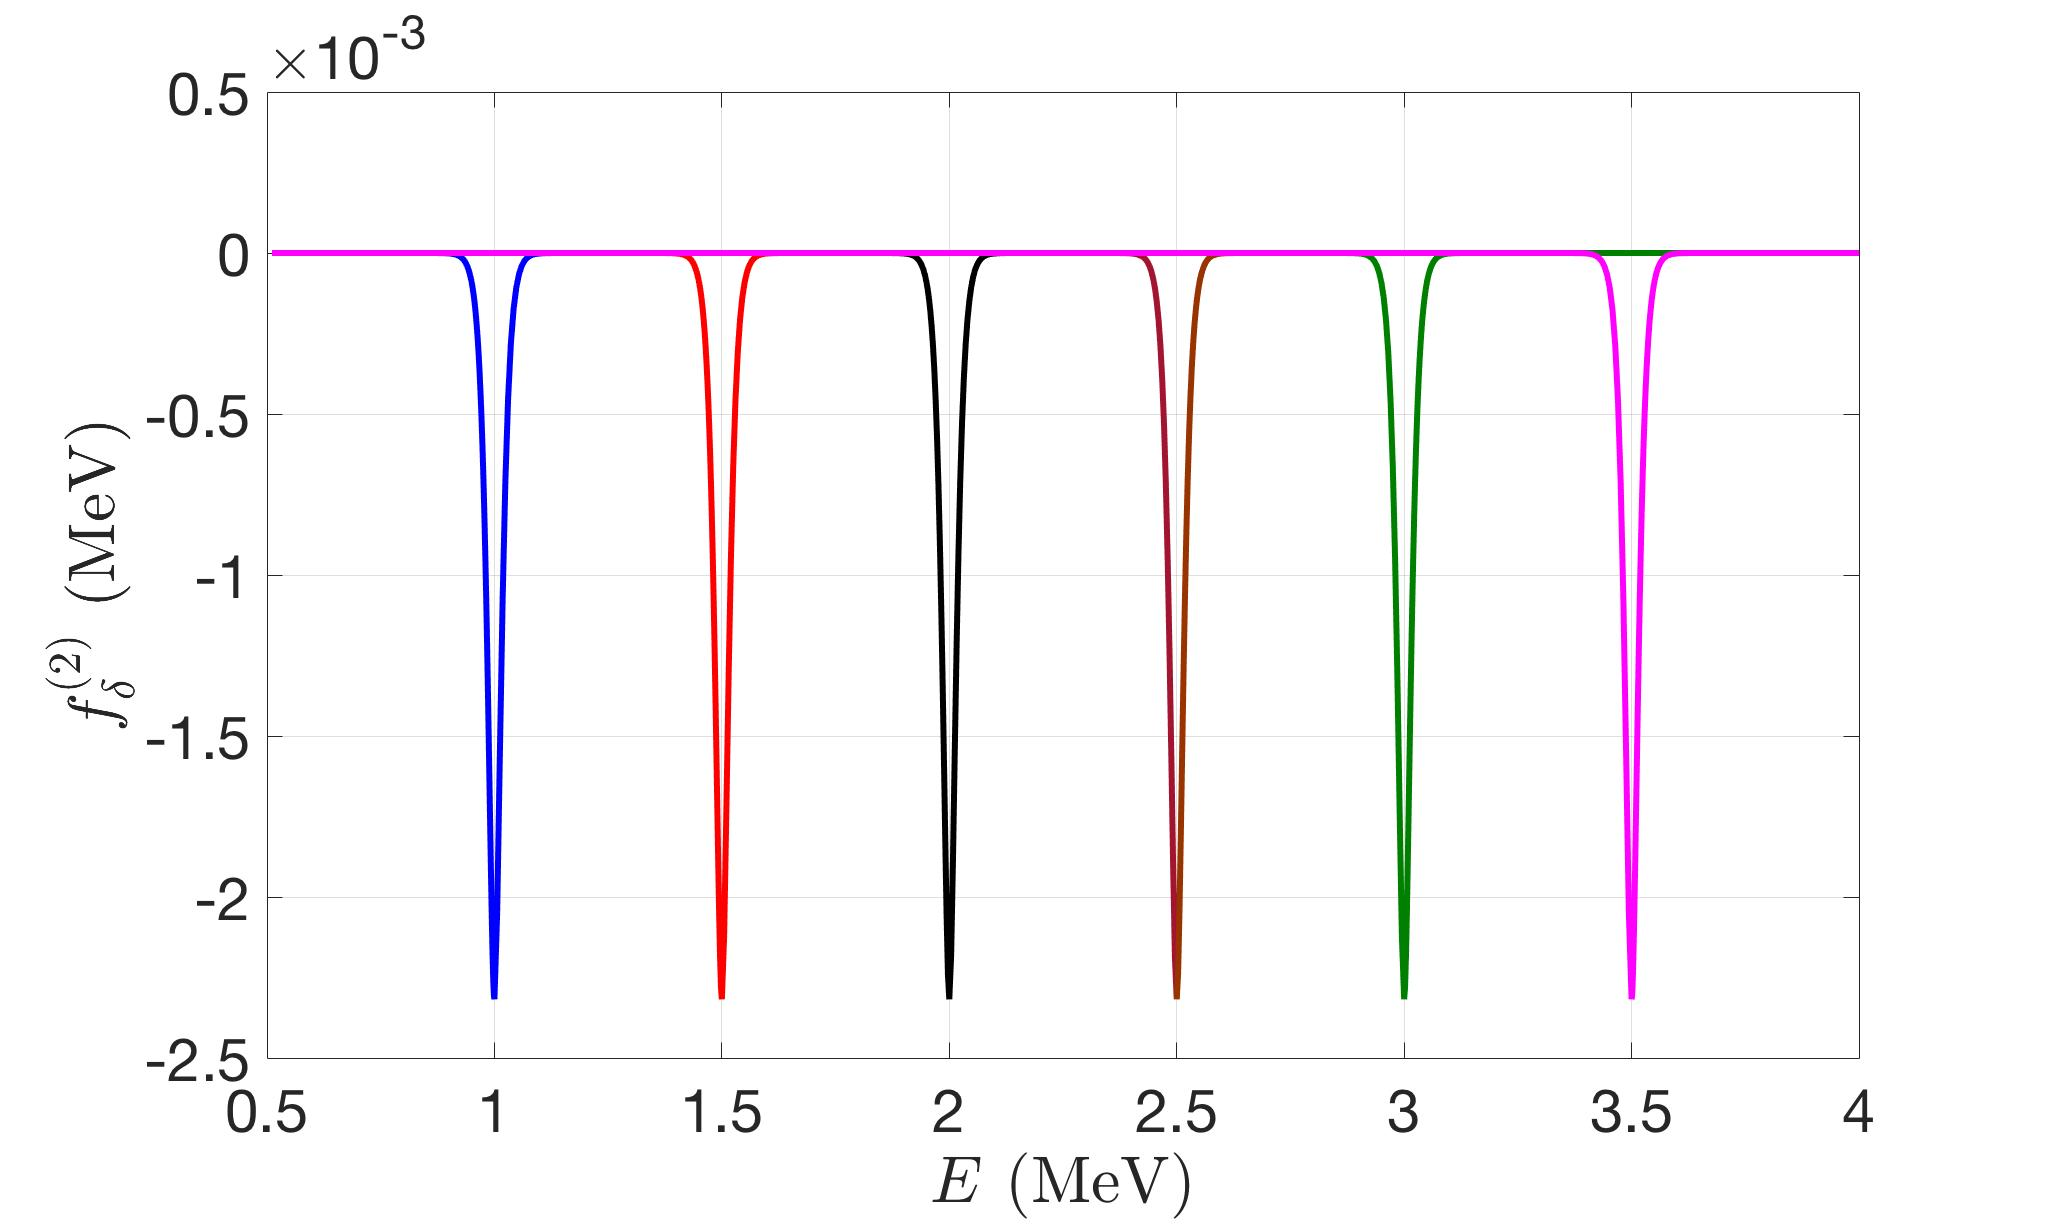
\includegraphics[width=0.9\textwidth]{./plot/f_delta_checking2}
\caption{We plot the function $f^{(2)}_\delta$ as a function of energy $E$ with $T=0.012\,\mathrm{MeV}$. We found that the behavier of $f^{(2)}_\delta$  is like delta function with peak at $E=\tilde\mu$. We have  $\tilde\mu=1.0\,\mathrm{MeV}, 1.5\,\mathrm{MeV}, 2.0\,\mathrm{MeV},2.5\,\mathrm{MeV}, 3.0\,\mathrm{MeV}, 3.5\,\mathrm{MeV}$.}
\label{f_delta_checking}
\end{center}
\end{figure}
%~~~~~~~~~~~~~~~~~~~~~~~~~~~~~~~~~~~~~~~~~~~~~~~~~~~~~~~~~~~~~~~~~~~~~~~~~~~~~~~~~~~~~~~~~~~~~~~



\bmhead{Acknowledgments}

We thank Gordon Baym and John W. Clark for their encouragement to publish this result.


\bibliography{sn-bibliography}% common bib file
%% if required, the content of .bbl file can be included here once bbl is generated
%%\input sn-article.bbl


\end{document}
